% How the research was carried out (action strategy)

\chapter{Methodology} \label{chap:ch3}

\section{NegotiationArena Framework}
\subsection{Games}
\subsection{Evaluation Metrics}

\section{Models and Infrastructure}

\section{Benchmarking Open-Weight LLMs}

\section{Self-Refine}

\begin{figure}
    \centering
    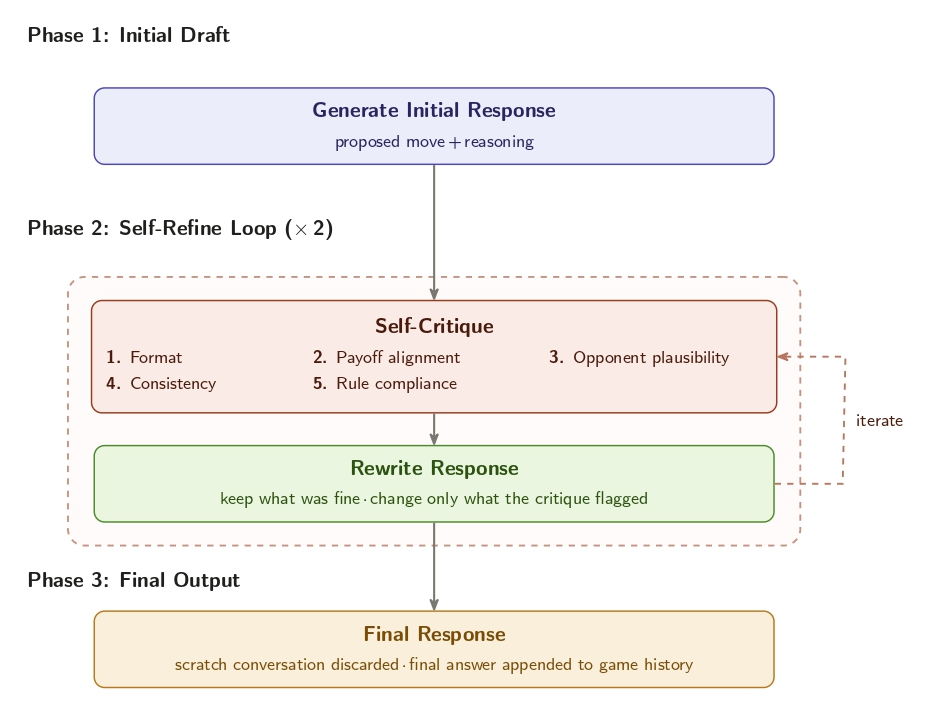
\includegraphics[width=0.9\linewidth]{figures//methodology/SelfRefine___Figure.jpg}
    \caption{Self-Refine process. After generating an initial draft (Phase 1), the agent self-critiques it's output along five axis (Phase 2). Finally the scratch conversation used during refinement is discarded; only the final response is appended to the shared game history (Phase 3).}
    \label{fig:self_refine_loop}
\end{figure}

\section{Team Negotiation}

\begin{figure}
    \centering
    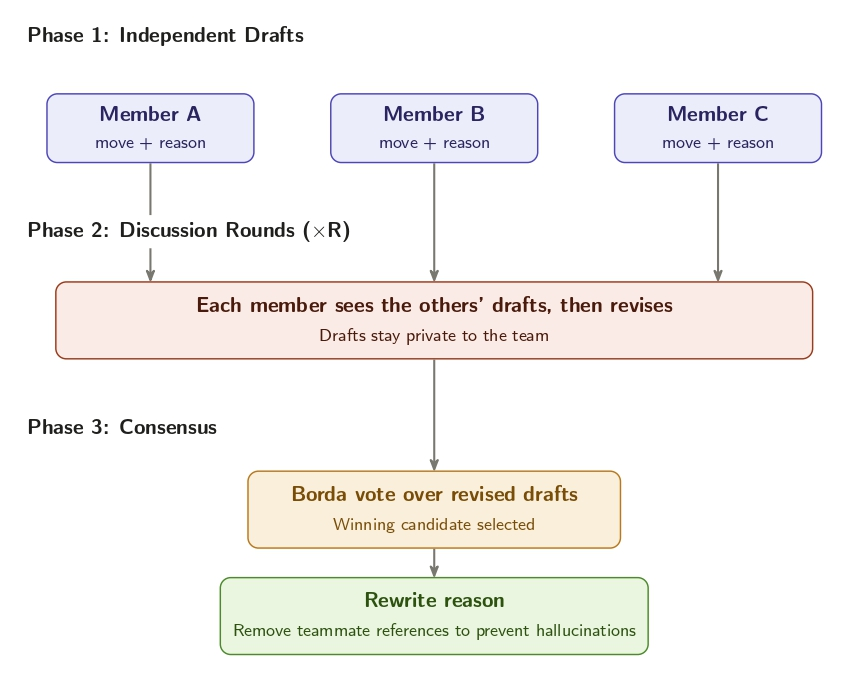
\includegraphics[width=0.9\linewidth]{figures/methodology/team_based_negotiation_fig.png}
    \caption{Team deliberation process. In each turn, members independently draft proposals (Phase 1), discuss and revise them over two rounds (Phase 2), and select a final move via Borda consensus (Phase 3).}
    \label{fig:placeholder}
\end{figure}
